Nous avons principalement tester que la fonction d'évaluation au niveau de l'application web et les fonctions utilisées dans notre solveur.

\subsection{Fonction d'évaluation de l'application web}

\subsubsection{Complexité théorique}

Soit n la longueur du mot choisi par le joueur; Soit k>0 est une constante.
Cette fonction a une complexité temporelle en o(k * $n$). La fonction d'évaluation a donc une complexité temporelle linéaire. 

\subsubsection{Graphe de performance}

On sait que, la complexité théorique de la fonction d'évaluation est linéaire. Sur cette figure qui mesure le temps d'exécution en fonction de la longueur des mots; On peut noter que le temps d'exécution croit linéairement avec une longueur croissante des mots. 
On peut donc confirmer la complexité théorique de cette fonction qui linéaire.

\begin{figure}[h!]
    \centering
    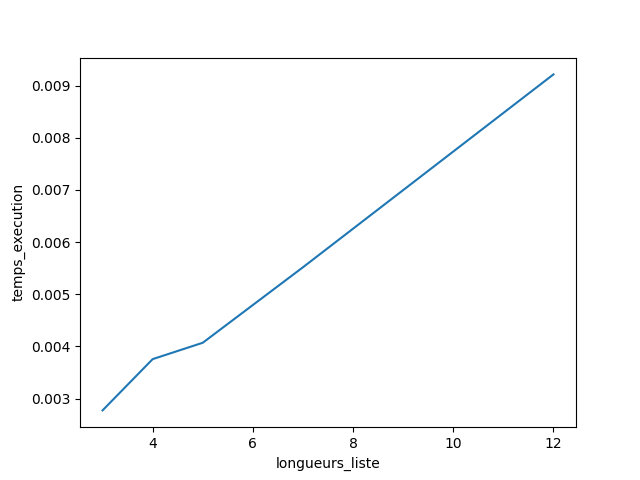
\includegraphics[scale=0.9]{figures/evaluation_test.png}
    \caption{Mesures du temps exécution en fonction de la longueur des mots}
    \label{fig:my_label}
\end{figure}
\newpage
\subsection{Fonction dicoload du solveur}
\subsubsection{Complexité théorique}
Soit p le nombre de mots du dictionnaire choisi, Cette fonction a une complexité temporelle en o($p$). La fonction dicoload du solveur a donc une complexité temporelle linéaire.

\subsection{Fonction evaluation du solveur}
\subsubsection{Complexité théorique}
Soit n la longueur des mots du dictionnaire choisi. Cette fonction a une complexité temporelle en o($n^2$). La fonction evaluation du solveur a donc une complexité temporelle quadratique.


\subsection{Fonction WordEntropy du solveur}
\subsubsection{Complexité théorique}
Soit p le nombre de mots du dictionnaire et n la longueur des mots; Cette fonction a une complexité temporelle en o(p * $n^2$).

\subsection{Fonction getbestword du solveur}
\subsubsection{Complexité théorique}
Soit p le nombre de mots du dictionnaire et n la longueur des mots; Cette fonction a une complexité temporelle en o($p^2$ * $n^2$).

\subsection{Fonction FindWordsGreen du solveur}
\subsubsection{Complexité théorique}
Soit p le nombre de mots du dictionnaire et n la longueur des mots; Cette fonction a une complexité temporelle en o($p$ * $n$).

\subsection{Fonction FindWordsYellow du solveur}
\subsubsection{Complexité théorique}
Soit p le nombre de mots du dictionnaire et n la longueur des mots; Cette fonction a une complexité temporelle en o($p$ * $n^2$).

\subsection{Fonction excludeWords du solveur}
\subsubsection{Complexité théorique}
Soit p le nombre de mots du dictionnaire et n la longueur des mots; Cette fonction a une complexité temporelle en o($p$ * $n^2$).

\subsection{Fonction MotsSuivantsPossibles du solveur}
\subsubsection{Complexité théorique}
Soit p le nombre de mots du dictionnaire et n la longueur des mots; Cette fonction a une complexité temporelle en o($p$ * $n^3$).